% ---------- Colours ----------
\colorlet{hat-colour}{black!20}
\colorlet{cardboard-colour}{brown!20}
\colorlet{circle-colour}{black}
\colorlet{teeth-colour}{black!40}
\begin{subfigure}{0.3\textwidth}
	\centering\begin{tikzpicture}
		\def\SquareLength{2} % Half the with of the top
		\def\CylLength{1} % Half the width of the cylinder
		\def\CylHeigth{2} % Height of the cylinder
		% Shift of the dimensions arrows <->
		\def\ShiftX{0.2}
		\def\ShiftY{0.3}
		% Position of coordinates:
		% ULL - UL - UR - URR
		%       LL - LR
		\coordinate (ULL) at (-\SquareLength, 0);
		\coordinate (UL) at (-\CylLength, 0);
		\coordinate (UR) at (\CylLength, 0);
		\coordinate (URR) at (\SquareLength, 0);
		\coordinate (LL) at (-\CylLength, -\CylHeigth);
		\coordinate (LR) at (\CylLength, -\CylHeigth);
		% Draw hat
		\draw[thick, fill=hat-colour] (UL) -- (UR) -- (LR) -- (LL) -- cycle;
		\draw[line width=1] (ULL) -- (URR);
		% Draw dimensioning
		\draw[<->] ($ (ULL) + (0,\ShiftY) $) -- ($ (URR) + (0,\ShiftY) $) node[midway, above]{$ S_1 $};
		\draw[<->] ($ (LL) + (0,-\ShiftY) $) -- ($ (LR) + (0,-\ShiftY) $) node[midway, below]{$ D $};
		\draw[<->, overlay] ($ (URR) + (\ShiftX, 0) $) -- ++(0, -\CylHeigth) node[midway, right]{$ H $};
	\end{tikzpicture}
	\caption{The finished hat from the side.}
	\label{fig:side}
\end{subfigure}%
% ---------- Parameters of the following two drawings ----------
\def\OuterSquareLength{2}% Side length of the outer square
\def\CircleRadius{0.55}% Radius of the cylinder circle
\def\nTeeth{20}% Number of teeth
\def\ToothRadius{0.35} % Radius of the (invisible) inner circle on which all ends of teeth lie
% ---------- Derived parameters of the drawings ----------
\pgfmathsetmacro{\ToothAngle}{360/\nTeeth}
\pgfmathsetmacro{\LastToothAngle}{360-\ToothAngle}
% ---------- Shifts for dimensioning ----------
\def\OuterSquareDimYShift{0.1}
\def\InnerSquareDimXShift{0.05}
\def\InnerSquareDimYShift{-0.05}
% ---------- Labels ----------
\def\OuterSquareLabel{$ S_2 $}
\def\InnerSquareLabel{$ S_1 $}
\def\DiameterLabel{$ D $}
\begin{subfigure}{0.3\textwidth}%
	\centering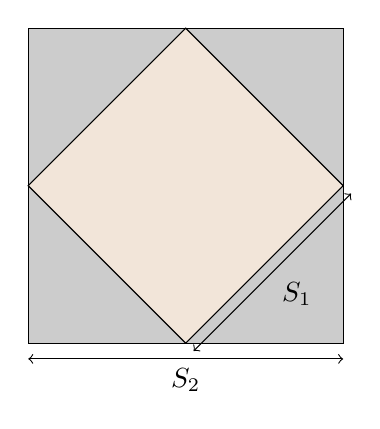
\begin{tikzpicture}[x=2cm,y=2cm]
		\coordinate (circle-mid) at (\OuterSquareLength/2, \OuterSquareLength/2);
		
		% Outer square
		\draw[fill=hat-colour] (0,0) rectangle (\OuterSquareLength, \OuterSquareLength);
		% Inner square
		\draw[fill=cardboard-colour] (\OuterSquareLength/2, 0) -- (\OuterSquareLength, \OuterSquareLength/2) -- (\OuterSquareLength/2, \OuterSquareLength) -- (0, \OuterSquareLength/2) -- cycle;
		
		% ---------- Dimensioning ----------
		% Outer square
		\draw[<->, shift={(0,-\OuterSquareDimYShift)}] (0,0) -- (\OuterSquareLength,0) node[midway,below]{\OuterSquareLabel};
		% Inner square
		\draw[<->, shift={(\InnerSquareDimXShift, \InnerSquareDimYShift)}] (\OuterSquareLength/2, 0) -- (\OuterSquareLength, \OuterSquareLength/2) node[midway, below right]{\InnerSquareLabel};
	\end{tikzpicture}%
	\caption{Gluing~\ref{black-square} onto~\ref{cardboard}.}%
	\label{fig:squares}
\end{subfigure}%
\begin{subfigure}{0.33\textwidth}
	\centering\begin{tikzpicture}[x=2cm,y=2cm]%[line width=0.8pt]
		\coordinate (circle-mid) at (\OuterSquareLength/2, \OuterSquareLength/2);
		
		% Inner square
		\draw[fill=hat-colour] (\OuterSquareLength/2, 0) -- (\OuterSquareLength, \OuterSquareLength/2) -- (\OuterSquareLength/2, \OuterSquareLength) -- (0, \OuterSquareLength/2) -- cycle;
		% Teeth
		\pgfmathsetmacro{\LastNumber}{\nTeeth-1}
		\foreach \x in {0, 1, ..., \LastNumber}{
			\pgfmathsetmacro{\StartAngle}{\x*\ToothAngle}
			\pgfmathsetmacro{\MidAngle}{(\x+0.5)*\ToothAngle}
			\pgfmathsetmacro{\EndAngle}{(\x+1)*\ToothAngle}
			
			\draw[fill=teeth-colour, shift=(circle-mid)] (\StartAngle:\CircleRadius) arc[start angle=\StartAngle, end angle=\EndAngle, radius=\CircleRadius] -- (\MidAngle:\ToothRadius) -- cycle;
		}
		% Circle
		\draw[thick, circle-colour] (circle-mid) circle[radius=\CircleRadius];
		
		% ---------- Dimensioning ----------
		% Inner square
		\draw[<->, shift={(\InnerSquareDimXShift, \InnerSquareDimYShift)}] (\OuterSquareLength/2, 0) -- (\OuterSquareLength, \OuterSquareLength/2) node[midway, below right]{\InnerSquareLabel};
		% Diameter
		\draw[<->, shift=(circle-mid)] (-\CircleRadius,0) -- (\CircleRadius,0) node[midway,below]{\DiameterLabel};
	\end{tikzpicture}%
	\caption{The finished hat from below.}
	\label{fig:below}
\end{subfigure}
